\documentclass[a4paper,twoside,onecolumn,openany,article,10pt]{memoir}
\usepackage{xeCJK}
\usepackage{url}
\usepackage{hyperref}
\usepackage{amsmath}
\usepackage{amssymb}
\usepackage{amsthm}
\usepackage{enumerate}
%\usepackage{algorithm}
%\usepackage{algorithmicx}
%\usepackage{algpseudocode}
\usepackage{ascmac}
\usepackage{tikz}
\usepackage{ulem}
%\usepackage{stix}
%\usepackage{bm}
\defaultfontfeatures{Ligatures=TeX}

\setCJKmainfont[BoldFont=Noto Sans CJK JP Bold]{Noto Serif CJK JP}
%\setCJKmainfont{Noto Serif CJK JP}
\setCJKsansfont{Noto Sans CJK JP}
\setCJKmonofont{Noto Sans Mono CJK JP}

\newtheorem{theorem}{定理}
\theoremstyle{remark}
\newtheorem{remark}{\textbf{余談}}


%\setmainfont{DejaVu Serif}
%\setsansfont{URW Gothic}
%\setmainfont{Noto Serif CJK JP}
\setmainfont[BoldFont=Noto Sans CJK JP Bold]{Noto Serif CJK JP}
\setsansfont{Noto Sans CJK JP}
\setmonofont{Inconsolata}

\usepackage{listings}

%\renewcommand{\algorithmcfname}{アルゴリズム}



\settrimmedsize{\stockheight}{\stockwidth}{*}

%\setlrmarginsandblock{1.5in}{1in}{*}
\setlrmarginsandblock{1.2in}{1.2in}{*}
\setulmarginsandblock{1.2in}{1.5in}{*}
\setheadfoot{20mm}{15mm}

%\newlength{\linespace}
%\setlength{\linespace}{\baselineskip}
%\setlength{\headheight}{\onelineskip}
%\setlength{\headsep}{\linespace}
%\addtolength{\headsep}{-\topskip}

%\setlength{\footskip}{\onelineskip}
%\setlength{\footnotesep}{\onelineskip}

\checkandfixthelayout

\counterwithout{section}{chapter}
\setsecnumdepth{subsubsection}


\title{アルゴリズムとデータ構造\\\vspace{.5em} \Large 二分探索}
\date{2018年6月15日}
\author{森~立平\\ \texttt{mori@c.titech.ac.jp}}

\begin{document}
\maketitle


\noindent
今日のメッセージ
\begin{itemize}
\item \textbf{ソートしてある配列から値を探すときは二分探索}
\item \textbf{二分探索の時間計算量は$O(\log n)$}
\end{itemize}

%\noindent
%今日の演習の目標
%\begin{itemize}
%\item 二分探索のプログラムを再帰、反復の両方で書けるようになる
%\end{itemize}
%
%\noindent
%今日の主な演習課題(提出締切は)
%\begin{enumerate}
%\item 二分探索のプログラムを書く
%\end{enumerate}
%
%\noindent
%今日の演習時間のワークフロー
%\begin{enumerate}
%\item GitHub のアカウントを取得し、Google Form で情報を送る(配布資料参照)
%\item \url{https://github.com/alg2018/} にアクセスし、\texttt{Algorithms--Datastructures}の「プログラミング演習のルール」を読む
%\item \url{https://github.com/alg2018/} にアクセスし、\texttt{GCD}にある課題に取り組む
%\item プログラムを紙に書いて教員かTAに提出
%\item \texttt{Algorithms--Datastructures/docs/git.pdf} を見て、\texttt{git}の使い方を覚える(来週以降に\texttt{git}を使用する)
%\end{enumerate}

\section{時間計算量のオーダー}
アルゴリズムの計算量は通常オーダー記法$O(\cdot)$を用いて表わす。
$f(n) = O(g(n)) \stackrel{\mathrm{def}}{\iff} \exists c>0, \forall n\ge 1, f(n) \le c g(n)$ という意味である。
なので $n$ も $100000000000 n$も $O(n)$であるし、$\log n$ も $O(n)$ である(もちろん $\log n$ は $O(\log n)$でもある)。
最大公約数の計算をするユークリッドの互除法と binary GCD は両方とも $O(n^2)$ である($n$は入力長であり、最大公約数を計算したい整数の桁数)。
ただし、定数倍の差で binary GCD の方が通常のコンピュータで高速となる。

\section{二分探索}
ソートしてある整数の列$A_0\le A_1\le A_2\le \dotsb\le A_{n-1}$の中から、$x$以上である最小のものを見つける問題を考えよう。
便宜上$A_n := +\infty$と定義し、
\begin{equation*}
\mathrm{bsearch}(\ell, r) := \min\bigl\{i\in\{\ell,\ell+1,\dotsc,r-1,r\}\mid A_i\ge x\bigr\}
\end{equation*}
と定義すると、解きたい問題は$\mathrm{bsearch}(0,n)$である(もしも$A_0$から$A_{n-1}$に$x$以上のものが無ければ$\mathrm{bsearch}(0,n)=n$となる)。
「アルゴリズム$\approx$漸化式」であるから、漸化式を立てることを考えよう。
\begin{equation*}
\mathrm{bsearch}(\ell, r) =
\begin{cases}
\ell,& \text{if } \ell = r\\
\mathrm{bsearch}(\lfloor \frac{\ell + r}2\rfloor+1, r),& \text{if } A_{\lfloor\frac{\ell + r}2\rfloor} < x\\
\mathrm{bsearch}(\ell, \lfloor \frac{\ell + r}2\rfloor),& \text{otherwise.}
\end{cases}
\end{equation*}
この漸化式に基づいてアルゴリズムを設計できる。

\begin{lstlisting}[basicstyle=\ttfamily\normalsize,showstringspaces=false,language=C,frame=single]
int binary_search(int A[], int x, unsigned int l, unsigned int r){
  unsigned int m;
  if(l >= r) return r;
  m = (l + r) / 2; // 桁溢れを考慮すると m = l + (r - l) / 2
  if(A[m] >= x) return binary_search(A, x, l, m);
  else return binary_search(A, x, m + 1, r);
}
\end{lstlisting}
便宜上$A_n=+\infty$として\textrm{bsearch}を定義したが、このアルゴリズムの中で\textbf{実際に$\mathtt{A[n]}$がアクセスされることはない}。

\section{二分探索の時間計算量}
一回の漸化式の適用で探索するべき候補は約半分になるので$O(\log n)$回(より具体的には$\lceil\log (n+1)\rceil$回)の漸化式の適用で停止する。

\section{反復による二分探索}
再帰によるプログラムを素直に反復に書き直すと次のようになる。
\begin{lstlisting}[basicstyle=\ttfamily\normalsize,showstringspaces=false,language=C,frame=single]
unsigned int binary_search(int A[], int x, int n){
  unsigned int l = 0;
  unsigned int r = n;
  while(r > l){
    unsigned int m = (l + r) / 2;
    if(A[m] >= x) r = m;
    else l = m + 1;
  }
  return r;
}
\end{lstlisting}
これはこれで構わないが、少し覚えにくい。二分探索はとても簡単なアルゴリズムだが\textbf{正確に書くのは難しい}(誰でも一度はバグらせたことがある)。
次のようなプログラムを覚えるとよい。
\begin{lstlisting}[basicstyle=\ttfamily\normalsize,showstringspaces=false,language=C,frame=single]
unsigned int binary_search(int A[], int x, int n){
  int lb = -1;
  int ub = n;
  while(ub - lb > 1){
    int m = (lb + ub) / 2;
    if(A[m] >= x) ub = m;
    else lb = m;
  }
  return ub;
}
\end{lstlisting}
これらの変数には次のような意味がある。
\begin{itemize}
\item \texttt{lb}は「\texttt{A[lb] < x}であることが分かっている最大の数」
\item \texttt{ub}は「\texttt{A[ub] >= x}であることが分かっている最小の数」
\end{itemize}
まず\texttt{A[-1] = -$\infty$}と解釈して、\texttt{lb = -1; ub = n} と初期化する。
もし\texttt{ub == lb + 1} ならば、\texttt{ub}が解となる。
\texttt{ub > lb + 1} ならば、\texttt{m = (lb + ub) / 2} とおく。
ここで、\texttt{m > lb \&\& ub > m} が成り立つことに注意する。
よって、\texttt{A[-1]}や\texttt{A[n]}はアクセスされないし、\texttt{ub - lb}は1ステップで必ず減少する。


最後に$n=12,\, x = 17$とした場合の例を紹介する。

\begin{center}
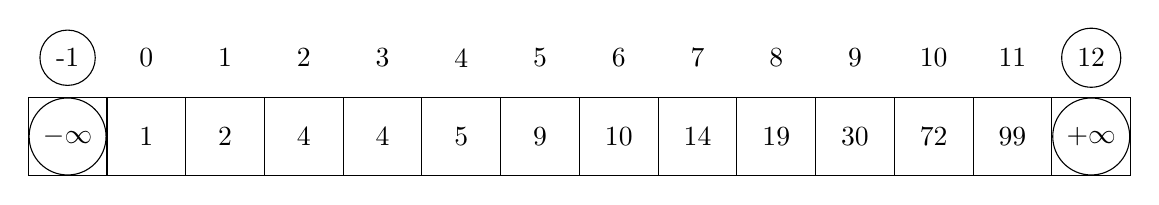
\begin{tikzpicture}
\draw[black] (-1,0) grid (13,1);
\node[circle,draw] at (-0.5,0.5) {$-\infty$};
\node at (0.5,0.5) {1};
\node at (1.5,0.5) {2};
\node at (2.5,0.5) {4};
\node at (3.5,0.5) {4};
\node at (4.5,0.5) {5};
\node at (5.5,0.5) {9};
\node at (6.5,0.5) {10};
\node at (7.5,0.5) {14};
\node at (8.5,0.5) {19};
\node at (9.5,0.5) {30};
\node at (10.5,0.5) {72};
\node at (11.5,0.5) {99};
\node[circle,draw] at (12.5,0.5) {$+\infty$};
\node[circle,draw] at (-0.5,1.5) {-1};
\node at (0.5,1.5) {0};
\node at (1.5,1.5) {1};
\node at (2.5,1.5) {2};
\node at (3.5,1.5) {3};
\node at (4.5,1.5) {4};
\node at (5.5,1.5) {5};
\node at (6.5,1.5) {6};
\node at (7.5,1.5) {7};
\node at (8.5,1.5) {8};
\node at (9.5,1.5) {9};
\node at (10.5,1.5) {10};
\node at (11.5,1.5) {11};
\node[circle,draw] at (12.5,1.5) {12};
\end{tikzpicture}
\end{center}

\begin{center}
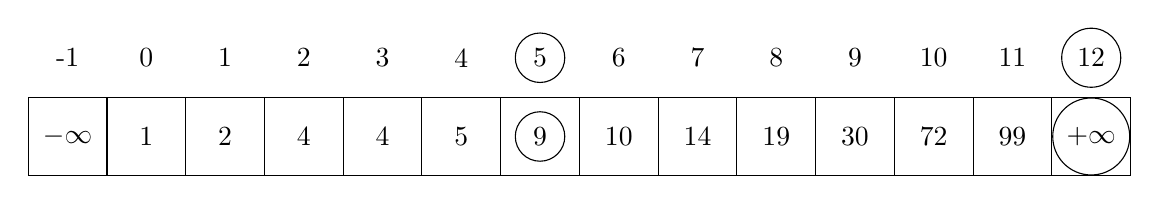
\begin{tikzpicture}
\draw[black] (-1,0) grid (13,1);
\node at (-0.5,0.5) {$-\infty$};
\node at (0.5,0.5) {1};
\node at (1.5,0.5) {2};
\node at (2.5,0.5) {4};
\node at (3.5,0.5) {4};
\node at (4.5,0.5) {5};
\node[circle,draw] at (5.5,0.5) {9};
\node at (6.5,0.5) {10};
\node at (7.5,0.5) {14};
\node at (8.5,0.5) {19};
\node at (9.5,0.5) {30};
\node at (10.5,0.5) {72};
\node at (11.5,0.5) {99};
\node[circle,draw] at (12.5,0.5) {$+\infty$};
\node at (-0.5,1.5) {-1};
\node at (0.5,1.5) {0};
\node at (1.5,1.5) {1};
\node at (2.5,1.5) {2};
\node at (3.5,1.5) {3};
\node at (4.5,1.5) {4};
\node[circle,draw] at (5.5,1.5) {5};
\node at (6.5,1.5) {6};
\node at (7.5,1.5) {7};
\node at (8.5,1.5) {8};
\node at (9.5,1.5) {9};
\node at (10.5,1.5) {10};
\node at (11.5,1.5) {11};
\node[circle,draw] at (12.5,1.5) {12};
\end{tikzpicture}
\end{center}

\begin{center}
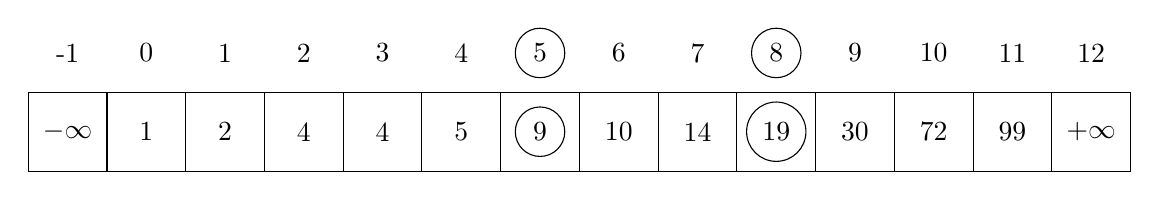
\begin{tikzpicture}
\draw[black] (-1,0) grid (13,1);
\node at (-0.5,0.5) {$-\infty$};
\node at (0.5,0.5) {1};
\node at (1.5,0.5) {2};
\node at (2.5,0.5) {4};
\node at (3.5,0.5) {4};
\node at (4.5,0.5) {5};
\node[circle,draw] at (5.5,0.5) {9};
\node at (6.5,0.5) {10};
\node at (7.5,0.5) {14};
\node[circle,draw] at (8.5,0.5) {19};
\node at (9.5,0.5) {30};
\node at (10.5,0.5) {72};
\node at (11.5,0.5) {99};
\node at (12.5,0.5) {$+\infty$};
\node at (-0.5,1.5) {-1};
\node at (0.5,1.5) {0};
\node at (1.5,1.5) {1};
\node at (2.5,1.5) {2};
\node at (3.5,1.5) {3};
\node at (4.5,1.5) {4};
\node[circle,draw] at (5.5,1.5) {5};
\node at (6.5,1.5) {6};
\node at (7.5,1.5) {7};
\node[circle,draw] at (8.5,1.5) {8};
\node at (9.5,1.5) {9};
\node at (10.5,1.5) {10};
\node at (11.5,1.5) {11};
\node at (12.5,1.5) {12};
\end{tikzpicture}
\end{center}

\begin{center}
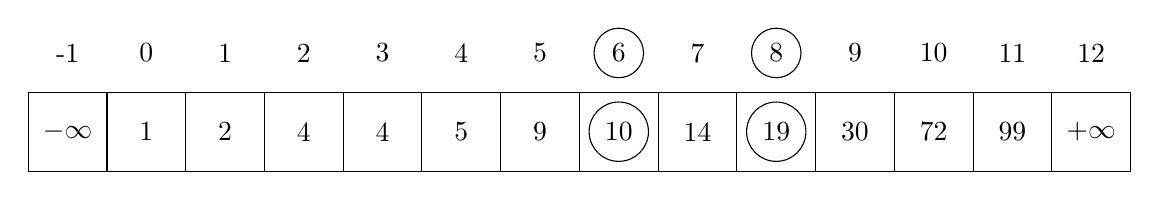
\begin{tikzpicture}
\draw[black] (-1,0) grid (13,1);
\node at (-0.5,0.5) {$-\infty$};
\node at (0.5,0.5) {1};
\node at (1.5,0.5) {2};
\node at (2.5,0.5) {4};
\node at (3.5,0.5) {4};
\node at (4.5,0.5) {5};
\node at (5.5,0.5) {9};
\node[circle,draw] at (6.5,0.5) {10};
\node at (7.5,0.5) {14};
\node[circle,draw] at (8.5,0.5) {19};
\node at (9.5,0.5) {30};
\node at (10.5,0.5) {72};
\node at (11.5,0.5) {99};
\node at (12.5,0.5) {$+\infty$};
\node at (-0.5,1.5) {-1};
\node at (0.5,1.5) {0};
\node at (1.5,1.5) {1};
\node at (2.5,1.5) {2};
\node at (3.5,1.5) {3};
\node at (4.5,1.5) {4};
\node at (5.5,1.5) {5};
\node[circle,draw] at (6.5,1.5) {6};
\node at (7.5,1.5) {7};
\node[circle,draw] at (8.5,1.5) {8};
\node at (9.5,1.5) {9};
\node at (10.5,1.5) {10};
\node at (11.5,1.5) {11};
\node at (12.5,1.5) {12};
\end{tikzpicture}
\end{center}

\begin{center}
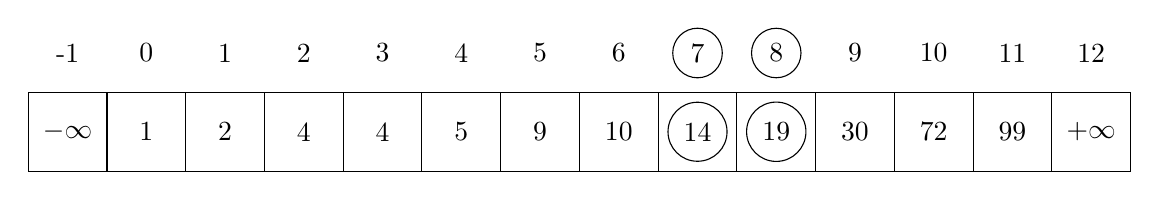
\begin{tikzpicture}
\draw[black] (-1,0) grid (13,1);
\node at (-0.5,0.5) {$-\infty$};
\node at (0.5,0.5) {1};
\node at (1.5,0.5) {2};
\node at (2.5,0.5) {4};
\node at (3.5,0.5) {4};
\node at (4.5,0.5) {5};
\node at (5.5,0.5) {9};
\node at (6.5,0.5) {10};
\node[circle,draw] at (7.5,0.5) {14};
\node[circle,draw] at (8.5,0.5) {19};
\node at (9.5,0.5) {30};
\node at (10.5,0.5) {72};
\node at (11.5,0.5) {99};
\node at (12.5,0.5) {$+\infty$};
\node at (-0.5,1.5) {-1};
\node at (0.5,1.5) {0};
\node at (1.5,1.5) {1};
\node at (2.5,1.5) {2};
\node at (3.5,1.5) {3};
\node at (4.5,1.5) {4};
\node at (5.5,1.5) {5};
\node at (6.5,1.5) {6};
\node[circle,draw] at (7.5,1.5) {7};
\node[circle,draw] at (8.5,1.5) {8};
\node at (9.5,1.5) {9};
\node at (10.5,1.5) {10};
\node at (11.5,1.5) {11};
\node at (12.5,1.5) {12};
\end{tikzpicture}
\end{center}

最終的に\texttt{ub == 8}となる。
\texttt{A[lb] < x} と \texttt{A[ub] >= x}が常に満たされていることに注意しよう。
\textbf{このように覚えておけば二分探索のプログラムを忘れることはない}。
二分探索はとても応用が広く、様々な問題を解くのに使うことができる。
その場合に特にこの覚えやすい二分探索の書き方が役に立つ。


\section{二分探索の応用}
二分探索はソートされた配列から値を探すという目的以外にも使用することができる。
ソートされた配列の代わりに単調な二値関数$p\colon \{0,1,2,\dotsc,n-1\}\to\{0,1\}$について考えよう。
ここで$p$が単調というのは$p(x)\ge p(x-1)$が$x=1,2,\dotsc,n-1$について満たされるという意味である。
このような$p$について
\begin{center}
$p(x) = 1$を満たす最小の$x\in\{0,1,2,\dotsc,n-1\}$をもとめよ
\end{center}
という問題を二分探索で解くことができる。
具体的には前節のプログラムのうち4行目からの5行を次のように変更すればよい。
\begin{lstlisting}[basicstyle=\ttfamily\normalsize,showstringspaces=false,language=C,frame=single]
while(ub - lb > l) {
  unsigned int m = (lb + ub) / 2;
  if(p(m)) ub = m;
  else lb = m;
}
\end{lstlisting}
実際に変更したのはこの中の3行目の\texttt{if}文の条件だけである。
この考え方を用いると、上記の問題について非常に大きな$n$に対しても現実的な時間で解くことができる。

例えば簡単な例として整数$n$の平方根の切り上げ$\lceil \sqrt{n}\rceil$を求める問題を考えよう。
この場合、
\begin{equation*}
p(x) :=
\begin{cases}
0,& \text{if } x < \lceil\sqrt{n}\rceil\\
1,& \text{if } x \ge \lceil\sqrt{n}\rceil
\end{cases}
\end{equation*}
となる。これは$x$が整数だとすると、次のように書き換えることができる。
\begin{equation*}
p(x) =
\begin{cases}
0,& \text{if } x^2 < n\\
1,& \text{if } x^2 \ge n
\end{cases}
\end{equation*}
この場合、
\begin{lstlisting}[basicstyle=\ttfamily\normalsize,showstringspaces=false,language=C,frame=single]
int p(unsigned int x){
  return x * x >= n;
}
\end{lstlisting}
と定義してあげれば、二分探索で$\lceil \sqrt{n}\rceil$が計算できる。
変数\texttt{lb}と\texttt{ub}の初期値は\texttt{lb = 0}, \texttt{ub = n}とすればよい(もちろん、もっと良い$\lceil\sqrt{n}\rceil$の上下界を使ってもよい)。
そうすると反復回数は$\lceil\log n\rceil$である。
このように、\textbf{簡単に計算ができる単調な関数の逆関数は二分探索を用いて計算ができる}。
ただし平方根の計算にはニュートン法というもっと効率的な方法が存在する。
しかしニュートン法は関数(この場合$x^2$にあたるもの)の凸性も用いるので、二分探索の方が適用範囲が広い。

\end{document}
